\documentclass[
11pt,
a4paper,
pdftex,
czech,
titlepage
]{report}

\usepackage[czech]{babel}
\usepackage[utf8]{inputenc}
\usepackage{lmodern}
\usepackage{textcomp}
\usepackage[T1]{fontenc}
\usepackage{amsfonts}
\usepackage{titlesec}
\usepackage{graphicx}
\usepackage[pdftex]{hyperref}
\usepackage[a4paper,left=30mm,right=30mm,top=28mm,bottom=30mm]{geometry}
\usepackage{enumitem}
\hypersetup{colorlinks=true,
  unicode=true,
  linkcolor=black,
  citecolor=black,
  urlcolor=black,
  bookmarksopen=true}

\titleformat{\chapter}
  {\normalfont\LARGE\bfseries}{\thechapter}{1em}{}
\titlespacing*{\chapter}{0pt}{0ex plus 1ex minus .2ex}{2.0ex plus .2ex}

\begin{document}

\begin{titlepage}
	%\vspace*{-2cm}
	{\centering
\includegraphics[scale=1.2]{logo-FAV.pdf}\par}
	\centering
	\vspace*{2.5cm}
	{\Large Semestrální práce z KIV/ZOS\par}
	\vspace{1.5cm}
	{\Huge\bfseries Souborový systém pseudoNTFS\par}
	\vspace{2.5cm}

	{\Large Zdeněk Častorál\par}
	{\Large A16B0467P\par}
	{\Large zcastora@students.zcu.cz\par}

	\vfill

	{\Large 4.\,2.\,2019}
\end{titlepage}

\tableofcontents
\thispagestyle{empty}
\clearpage

\chapter{Zadání}\label{intro}
\setcounter{page}{3}
Tématem semestrální práce je návrh a implementace souborového systému pseudoNTFS. Vytvořený souborový systém bude umožňovat vykonávání základních příkazů nad soubory a adresáři. Jedná se například o vytvoření adresáře, kopírování souborů, přesouvání souborů atd.

Program se bude spouštět s jedním parametrem a tím bude název souborového systému (např. \texttt{myFS}). Po spuštění bude program čekat na zadání jednotlivých příkazů (všechny soubory mohou být zadány jak absolutní, tak relativní cestou).

Práce bude realizována v jazyce \textit{C/C++}.\\[0.5\baselineskip]
\noindent Jednotlivé příkazy nad souborovým systémem jsou uvedeny níže.

\begin{enumerate}[label=\textbf{\arabic*}.]
\item \textbf{Zkopíruje soubor s1 do umístění s2.}\\[0,2cm]
\noindent \framebox{\texttt{cp s1 s2}}\\[0.5\baselineskip]
Možný výsledek:\\
\texttt{OK}\\
\texttt{FILE NOT FOUND} (není zdroj)\\
\texttt{PATH NOT FOUND} (neexistuje cílová cesta)\\

\item \textbf{Přesune soubor s1 do umístění s2.}\\[0,2cm]
\noindent \framebox{\texttt{mv s1 s2}}\\[0.5\baselineskip]
Možný výsledek:\\
\texttt{OK}\\
\texttt{FILE NOT FOUND} (není zdroj)\\
\texttt{PATH NOT FOUND} (neexistuje cílová cesta)\\

\item \textbf{Smaže soubor s1.}\\[0,2cm]
\noindent \framebox{\texttt{rm s1}}\\[0.5\baselineskip]
Možný výsledek:\\
\texttt{OK}\\
\texttt{FILE NOT FOUND}\\

\item \textbf{Vytvoří adresář a1.}\\[0,2cm]
\noindent \framebox{\texttt{mkdir a1}}\\[0.5\baselineskip]
Možný výsledek:\\
\texttt{OK}\\
\texttt{PATH NOT FOUND} (neexistuje zadaná cesta)\\
\texttt{EXIST} (nelze založit, již existuje)\\

\item \textbf{Smaže prázdný adresář a1.}\\[0,2cm]
\noindent \framebox{\texttt{rmdir a1}}\\[0.5\baselineskip]
Možný výsledek:\\
\texttt{OK}\\
\texttt{FILE NOT FOUND} (neexistující adresář)\\
\texttt{NOT EMPTY} (adresář obsahuje podadresáře, nebo soubory)\\

\item \textbf{Vypíše obsah adresáře a1.}\\[0,2cm]
\noindent \framebox{\texttt{ls a1}}\\[0.5\baselineskip]
Možný výsledek:\\
\texttt{-FILE}\\
\texttt{+DIRECTORY}\\
\texttt{PATH NOT FOUND} (neexistující adresář)\\

\item \textbf{Vypíše obsah souboru s1.}\\[0,2cm]
\noindent \framebox{\texttt{cat s1}}\\[0.5\baselineskip]
Možný výsledek:\\
\texttt{OBSAH}\\
\texttt{FILE NOT FOUND} (není zdroj)\\

\item \textbf{Změní aktuální cestu do adresáře a1.}\\[0,2cm]
\noindent \framebox{\texttt{cd a1}}\\[0.5\baselineskip]
Možný výsledek:\\
\texttt{OK}\\
\texttt{PATH NOT FOUND} (neexistující cesta)\\

\item \textbf{Vypíše aktuální cestu.}\\[0,2cm]
\noindent \framebox{\texttt{pwd}}\\[0.5\baselineskip]
Možný výsledek:\\
\texttt{PATH}\\

\item \textbf{Vypíše informace o souboru/adresáři s1/a1 (v jakých fragmentech/clusterech se nachází), uid, …}\\[0,2cm]
\noindent \framebox{\texttt{info a1/s1}}\\[0.5\baselineskip]
Možný výsledek:\\
\texttt{NAME – UID – SIZE - FRAGMENTY - CLUSTERY}\\
\texttt{FILE NOT FOUND} (není zdroj)\\

\item \textbf{Nahraje soubor s1 z pevného disku do umístění s2 v pseudoNTFS.}\\[0,2cm]
\noindent \framebox{\texttt{incp s1 s2}}\\[0.5\baselineskip]
Možný výsledek:\\
\texttt{OK}\\
\texttt{FILE NOT FOUND} (není zdroj)\\
\texttt{PATH NOT FOUND} (neexistuje cílová cesta)\\

\item \textbf{Nahraje soubor s1 z pseudoNTFS do umístění s2 na pevném disku.}\\[0,2cm]
\noindent \framebox{\texttt{outcp s1 s2}}\\[0.5\baselineskip]
Možný výsledek:\\
\texttt{OK}\\
\texttt{FILE NOT FOUND} (není zdroj)\\
\texttt{PATH NOT FOUND} (neexistuje cílová cesta)\\

\item \textbf{Načte soubor z pevného disku, ve kterém budou jednotlivé příkazy a začne je sekvenčně vykonávat. Formát je 1 příkaz/1řádek.}\\[0,2cm]
\noindent \framebox{\texttt{load s1}}\\[0.5\baselineskip]
Možný výsledek:\\
\texttt{OK}\\
\texttt{FILE NOT FOUND} (není zdroj)\\

\item \textbf{Příkaz provede formát souboru, který byl zadán jako parametr při spuštení programu na souborový systém dané velikosti. Pokud už soubor nějaká data obsahoval, budou přemazána. Pokud soubor neexistoval, bude vytvořen.}\\[0,2cm]
\noindent \framebox{\texttt{format 600MB}}\\[0.5\baselineskip]
Možný výsledek:\\
\texttt{OK}\\
\texttt{CANNOT CREATE FILE}\\

\item \textbf{Vytvoří symbolický link na soubor s1 s názvem s2. Dále se s ním pracuje očekávaným způsobem, tedy např. cat s2 vypíše obsah souboru s1.}\\[0,2cm]
\noindent \framebox{\texttt{slink s1 s2}}\\[0.5\baselineskip]
Možný výsledek:\\
\texttt{OK}\\
\texttt{FILE NOT FOUND} (není zdroj)\\
\texttt{PATH NOT FOUND} (neexistuje cílová cesta)\\
\end{enumerate}

\noindent Budeme předpokládat korektní zadání syntaxe příkazů, nikoliv však sémantiky (tj. např. cp s1 zadáno nebude, ale může být zadáno cat s1, kde s1 neexistuje).


\chapter{Programátorská dokumentace}
\section{Struktura NTFS}
\textit{Souborový systém NTFS} se skládá ze 4 hlavních částí (viz obrázek \ref{ntfs_struct}).\\

\begin{figure}[!ht]
	\centering
	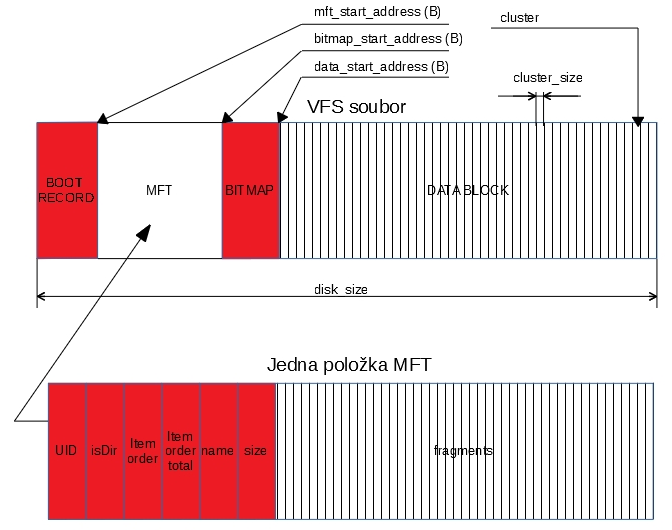
\includegraphics[width=1\textwidth]{img/zos-ntfs.png}
	\caption{Struktura souborového systému NTFS}
	\label{ntfs_struct}
\end{figure}

\noindent Části souborového systému NTFS jsou:
\begin{itemize}
\item \textbf{boot record}:
	\begin{itemize}
	\item uchovává informace o celém souborovém systému, např. název, popis, velikost, adresa počátku MFT záznamů, adresa počátku bitmapy atd.,
	\item je umístěn na začátku oblasti vymezené pro souborový systém,
	\end{itemize}
\item \textbf{MFT záznamy}:
	\begin{itemize}
	\item spravují informace o souborech,
	\item každý záznam obsahuje: unikátní číslo, typ položky: soubor/adresář/..., název souboru, velikost souboru, pořadí záznamu, celkový počet záznamů, popis fragmentů,
	\item MFT záznamy jsou umístěny za boot recordem,
	\end{itemize}
\item \textbf{bitmapa}:
	\begin{itemize}
	\item spravuje informace datové části -- které bloky jsou volné a které obsazené,
	\item velikost bitmapy se rovná počtu clusterů datové části souborového systému,
	\item bitmapa je umístěna za MFT záznamy,
	\end{itemize}
\item \textbf{datová část}:
	\begin{itemize}
	\item v datové části jsou fyzicky uložena data souborů,
	\item je rozdělena na clustery pevné velikosti,
	\item datová část je umístěna za bitmapou a je tak poslední částí souborového systému.
	\end{itemize}
\end{itemize}

\section{Realizace programu}
Program je dle zadání implementován v jazyce C a odladěn pro fungování v prostředí operačních systémů \textit{Windows}. Konkrétně byl program vyvíjen a laděn na systému \textit{Windows 10 Enterprise}, k překladu byl použit překladač \texttt{gcc 4.9.2}.

Aplikace je rozdělena do několika modulů, které jsou blíže popsány v kapitole \ref{moduls}.

\subsection{Moduly programu}\label{moduls}
Program je rozdělen do devíti modulů a osmi hlavičkových souborů, které jednotlivým modulům přísluší.

\begin{itemize}
\item Modul \texttt{main.c} (nemá svůj hlavičkový soubor):
	\begin{itemize}
	\item je hlavním modulem programu,
	\item sjednocuje všechny komponenty programu (moduly a hlavičkové soubory) a obsahuje spustitelný bod programu,
	\item zpracovává argumenty příkazové řádky,
	\item připravuje program pro ukončení (zavření proudů, uvolnění paměti atd.).
	\end{itemize}
\item Modul \texttt{shell.c} (jeho hlavičkový soubor -- \texttt{shell.h}):
	\begin{itemize}
	\item reprezentuje shell, který zpracovává vstup od uživatele,
	\item žádá ostatní komponeny programu o zpracování požadavku.
	\end{itemize}
\item Modul \texttt{command.c} (jeho hlavičkový soubor -- \texttt{command.h}):
	\begin{itemize}
	\item slouží k rozdělení vstupu od uživatele na \textit{příkaz} a \textit{parametry},
	\item také slouží jako přepravka těchto hodnot.
	\end{itemize}
\item Modul \texttt{process\_command.c} (jeho hlavičkový soubor -- \texttt{process\_command.h}):
	\begin{itemize}
	\item slouží ke zpracování jednotlivých příkazů,
	\item volá příslušné funkce pro vykonání požadované funkcionality zadaného příkazu.
	\end{itemize}
\item Modul \texttt{functions.c} (jeho hlavičkový soubor -- \texttt{functions.h}):
	\begin{itemize}
	\item obsahuje funkce pro vykonávání jednotlivých funkcí shellu,
	\item funkce tohoto modulu jsou volány modulem \texttt{process\_command.c},
	\item funkce tohoto modulu využívají funkce modulu \texttt{functions\_helper.c}.
	\end{itemize}
\item Modul \texttt{functions\_helper.c} (jeho hlavičkový soubor -- \texttt{functions\_helper.h}):
	\begin{itemize}
	\item obsahuje pomocné funkce pro realizaci funkcí pro vykonávání jednotlivých příkazů shellu,
	\item funkce tohoto modulu jsou volány moduly \texttt{process\_command.c} a  \texttt{functions.c}.
	\end{itemize}
\item Modul \texttt{file\_manager.c} (jeho hlavičkový soubor -- \texttt{file\_manager.h}):
	\begin{itemize}
	\item stará se o práci s datovým souborem pro uložení souborového systému,
	\item stará se o jeho vytvoření, uložení struktur, formátování atd.
	\end{itemize}
\item Modul \texttt{fs\_structures.c} (jeho hlavičkový soubor -- \texttt{fs\_structures.h}):
	\begin{itemize}
	\item vytváří struktury potřebné pro souborový systém,
	\item obsahuje funkce pro základní operace s těmito strukturami.
	\end{itemize}
\item Modul \texttt{global\_vars.c} (jeho hlavičkový soubor -- \texttt{global\_vars.h}):
	\begin{itemize}
	\item reprezentuje přepravku pro globální proměnné celé aplikace.
	\end{itemize}
\end{itemize}

\subsection{Běh programu}
Program se spouští s jedním parametrem, který obsahuje název souborového systému -- například \texttt{myFS}. 

Při prvním spuštění tento soubor zatím neexistuje, je nutné jej vytvořit a zformátovat. Zadáním příkazu \texttt{format 600MB} se vytvoří soubor, jehož název je zadán v parametru, a připraví ho k použití. V této fázi je již možné používat všechny příkazy implementované nad souborovým systémem (viz kapitola \ref{intro}).

Při dalším spuštění již bude soubor existovat a bude obsahovat námi vytvořené soubory a adresáře a dojde pouze k načtení obsahu do programu.

\subsection{Příkazy programu}
Jednotlivé příkazy nad souborovým systémem jsou podrobně uvedeny v kapitole \ref{intro}.\\[0.5\baselineskip]
\noindent Stručný přehled příkazů:
\begin{itemize}
\item \texttt{cp s1 s2} -- zkopíruje soubor \texttt{s1} do umístění \texttt{s2},
\item \texttt{mv s1 s2} -- přesune soubor \texttt{s1} do umístění \texttt{s2},
\item \texttt{rm s1} -- smaže soubor \texttt{s1},
\item \texttt{mkdir a1} -- vytvoří adresář \texttt{a1},
\item \texttt{rmdir a1} -- smaže prázdný adresář \texttt{a1},
\item \texttt{ls a1} -- vypíše obsah adresáře \texttt{a1},
\item \texttt{cat s1} -- vypíše obsah souboru \texttt{s1},
\item \texttt{cd a1} -- změní aktuální cestu do adresáře \texttt{a1},
\item \texttt{pwd} -- vypíše aktuální cestu,
\item \texttt{info a1/s1} -- vypíše informace o adresáři/souboru,
\item \texttt{incp s1 s2} -- nahraje soubor \texttt{s1} z pevného disku do umístění \texttt{s2} v pseudoNTFS,
\item \texttt{outcp s1 s2} -- nahraje soubor \texttt{s1} z pseudoNTFS do umístění \texttt{s2} na pevném disku,
\item \texttt{load s1} -- sekvenčně vykoná příkazy umístěné v souboru \texttt{s1} na pevném disku,
\item \texttt{format} \textit{<velikost>} \texttt{MB} -- zformátuje soubor na zadanou velikost,
\item \texttt{slink s1 s2} -- vytvoří symbolický link na soubor \texttt{s1} s názvem \texttt{s2},
\item \texttt{exit} -- uvolní paměť, zavře proudy a ukončí program.
\end{itemize}

\subsubsection{Příkaz \texttt{slink}}
Příkaz \texttt{slink s1 s2} vytvoří symbolický link na soubor \texttt{s1} s názvem \texttt{s2}. Symbolický link lze vytvořit pouze mezi obyčejnými soubory.\\[0.5\baselineskip]
\noindent Nad symbolickým linkem lze vykonávat následující příkazy:
\begin{itemize}
\item \texttt{cp s1 s2} -- vytvoří kopii symbolického linku \texttt{s1} do umístění \texttt{s2} (bude odkazovat na stejný soubor),
\item \texttt{mv s1 s2} -- přesune symbolický link \texttt{s1} do umístění \texttt{s2},
\item \texttt{rm s1} -- smaže symbolický link \texttt{s1},
\item \texttt{cat s1} -- vypíše obsah souboru, na který odkazuje symbolický link \texttt{s1},
\item \texttt{info s1} -- vypíše informace o symbolickém linku \texttt{s1},
\item \texttt{outcp s1 s2} -- nahraje soubor, na který odkazuje symbolický link \texttt{s1}, do umístění \texttt{s2} na pevném disku.\\
\end{itemize}

\noindent Symbolický link je implementován tak, že v MFT záznamu je vytvořen speciální typ položky: \textit{symbolický link}. Tento typ položky obsahuje pouze jeden fragment délky $1$, protože v datové části je uloženo pouze UID souboru (\texttt{integer} -- 4 byty), na který symbolický link odkazuje, a ukončovací hodnota $-1$  (\texttt{integer} -- 4 byty). Díky tomu je velikost symbolického linku vždy 8 bytů a v datové části pro něj postačuje jen jeden cluster.

\subsection{Překlad programu}
Pro jednoduchý překlad je v kořenovém adresáři programu vytvořen soubor \texttt{makefile}. Překlad je spuštěn zadáním příkazu \texttt{make} do \textit{Příkazového řádku}. Překlad je realizován překladačem \texttt{gcc}. 

K překlad je nutné mít nainstalovány programy: \texttt{make}, \texttt{gcc}.

\chapter{Uživatelská dokumentace}
V následující kapitole je popsáno supštění a ovládán souborového systému \textit{pseudoNTFS}.

\section{Spuštění programu}
Jedna z možných variant spuštění programu je popsána v následujících bodech:

\begin{enumerate}
\item otevřít \textit{Příkazový řádek} a dostat se do kořenového adresáře programu,
\item spustit program příkazem: \texttt{pseudoNTFS.exe} <\textit{souborový\_systém}>.\\
\end{enumerate}

\noindent Parametr <\textit{souborový\_systém}> je povinný. Jedná se o název souboru, do kterého bude ukládán souborový systém. Pokud bude program spuštěn bez parametru, program vypíše nápovědu o správném použití. Ilustrační příklad spuštění programu je zobrazen na obrázku \ref{start_prog}.

\begin{figure}[!ht]
	\centering
	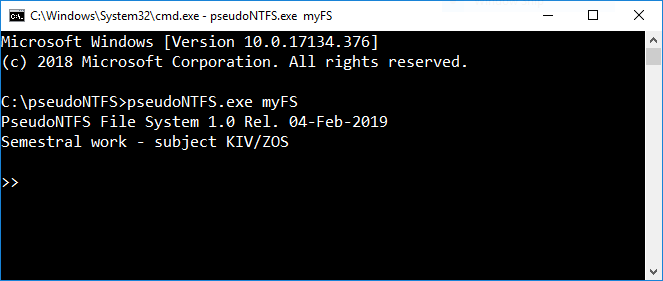
\includegraphics[width=1\textwidth]{img/start_prog.png}
	\caption{Příklad spuštění programu}
	\label{start_prog}
\end{figure}

\section{Ovládání programu}
Po úspěšném spuštění programu mohou nastat dvě možnosti: buď soubor předaný v parametru existuje, nebo neexistuje. 

V případě, že soubor neexistuje, je nutné jej nejprve vytvořit a zformátovat na počáteční hodnoty. O to se stará příkaz \texttt{format} <\textit{velikost}> \texttt{MB}. Po zformátování souboru je možné používat všechny příkazy uvedené v kapitole \ref{intro}.

Pokud již soubor, jehož název je předaný v parametru při spuštění programu, existuje, dojde k načtení obsahu tohoto souboru a je možné používat příkazy uvedené v kapitole \ref{intro} ihned.

Program je možné ukončit zadáním příkazu \texttt{exit}. Ilustrační příklad běhu programu je zobrazen na obrázku \ref{run_prog}.

\begin{figure}[!ht]
	\centering
	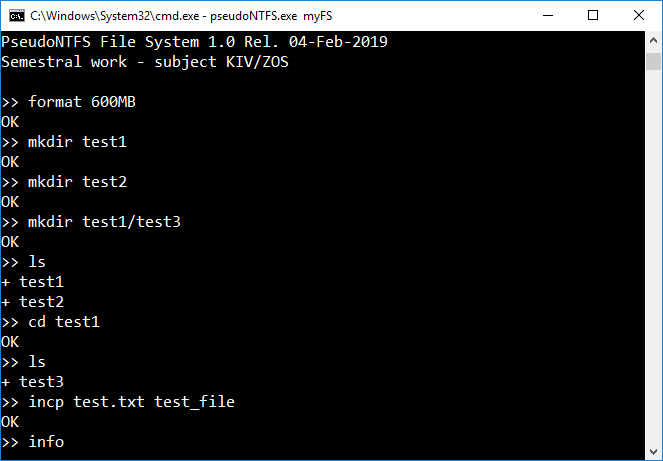
\includegraphics[width=1\textwidth]{img/run_prog.png}
	\caption{Příklad běhu programu}
	\label{run_prog}
\end{figure}


\chapter{Závěr}
\section{Testování}
Program byl testován na operačních systémech: 
\begin{itemize}
\item Windows 10 Enterprise,
\item Ubuntu 18.04.1 LTS (Bionic Beave),
\item Debian GNU/Linux 9 (stretch).\\
\end{itemize}

\noindent V rámci testování došlo například k porovnání, zda při importu a následném exportu daného souboru jsou oba soubory stejně velké. Dále jsem testoval schopnost programu vypořádat se s nevalidními vstupy od uživatele, nahrání velkých souborů do souborového systému a také nahrání velkého množství různě velkých souborů. Program ve zmíněných testech uspěl. 


\section{Zhodnocení práce}
Cílem semestrální práce bylo navrhnout a implementovat souborový systém pseudoNTFS, který bude umět zpracovávat základní příkazy nad soubory a adresáři (viz kapitola \ref{intro}).

Návrh a implementace řešení proběhly úspěšně. Při řešení této semestrální práce jsem se nesetkal s většimi problémy.\\

\noindent Semestrální práce z mého pohledu splňuje požadavky zadání.

\end{document}